\chapter{Wireless Channel Modeling}

% TODO: Introduce Fadnig impairments following
% Simulation of Communication Systems



% TODO: give the text book description of large scale fading
\newpage
\section{Fading Channels}

Fading is a major component of wireless channel %
impairments. Fading comes under two main categories %
large scale and small scale fading. Figure \ref{fig:Fading} %
illustrates these two main components of fading.
\FloatBarrier
\begin{figure}[h!]
	\centering
	\includegraphics[width=\textwidth,
		height=\textheight, keepaspectratio]
		{./Figures/%
		WirelessChannel/LargeandSmallScale%	
		Fading.png}
	\caption{combination of large and small %
		scale fading (a) and the small-scale %
		fading component (b) from %
		\cite{Sklar97-1}}
	\label{fig:Fading}
\end{figure}

\FloatBarrier
\subsection{Large Scale Fading}

Large scale fading, also sometimes referred to as %
shadow fading is characterised by an attenuation %
of the average signal power as can be seen in %
figure \ref{fig:Fading}a). It is caused %
by significant obstructions to the signal such as %
buildings or hills between the transmitter and %
receiver. The receiver is therefore being %
\emph{shadowed} by the obstruction. 

The received signal power can be modeled as:

\begin{align}
	S_{r} = S_{t} + G_{t} + G_{r} - L_{p}
\end{align}

Where $S_{r}$ is the received signal power in dB, %
$S_{t}$ is the transmit signal power in dB, $G_{t}$ 
and $G_{r}$ are the transmit and receive antenna %
gains in dB and $L_{p}$ is the propagation loss in dB. %
Typically $S_{r}$, $S_{t}$, $G_{t}$, and $G_{r}$ are %
either well known or are easily modeled, in the case of %
fading channels the propagation loss is the most difficult %
to predict \cite{Jer00}. There are two main methods %
of attempting to model $L_{p}$, ray tracing methods %
which must be location specific and statistical models. %
I will constrain this section to the development of %
statistical models. 

The most popular of the statistical models are the %
class of slope-intercept models \cite{Jer00}. These %
models treat propagation loss as being composed of %
a deterministic component and a statistical component.

\begin{align}
	L_{p} = \alpha + \beta log_{10}(R) + \gamma \text{ dB}
\end{align}

where $R$ is the distance from the transmitter to the %
receiver in kilometres, $\alpha$ and $\beta$ are parameters %
determined by the model, and $\gamma$ is the %
statistical component of the model. Values for $\alpha$ and %
$\beta$ are determined from experimental measurements %
where received signal power averaged over several %
wavelengths are taken over many different locations %
around the transmitter. These received signal %
powers can be plotted against the log of %
the distance to the transmitter and a least squares fit %
can be made to the data. The resulting residuals around %
the least squares fit describes $\gamma$.

Some well-known slope intercept models are the Hata%
\cite{Hata80} model and the COST-231 model\cite{COST231}.

Typically the residuals  of the slope intercept models %
when measured in dB follow a gaussian distribution with %
zero mean and a standard deviation of about 8dB\cite{Jer00}.
So the large scale fading follows a log-normal distribution.

\subsection{Small Scale Fading}
% TODO: give the textbook description of small scale fading

Small scale fading is caused by a transmitted signal %
arriving at the receiver with slightly different delays %
and angles after having been scattered or reflected by %
the environment in some way. The signals all self %
interfere at the receiver causing constructive or %
destructive interference. 

% TODO: make a diagram depicting the self interference

Small scale fading is typically modeled as having an %
envelope that follows a Rayleigh distribution or a %
Rician distribution, normally referred to as Rayleigh %
fading and Rician fading respectively. % TODO: maybe reference
% simulation of communication systems


\begin{figure}[h!]
	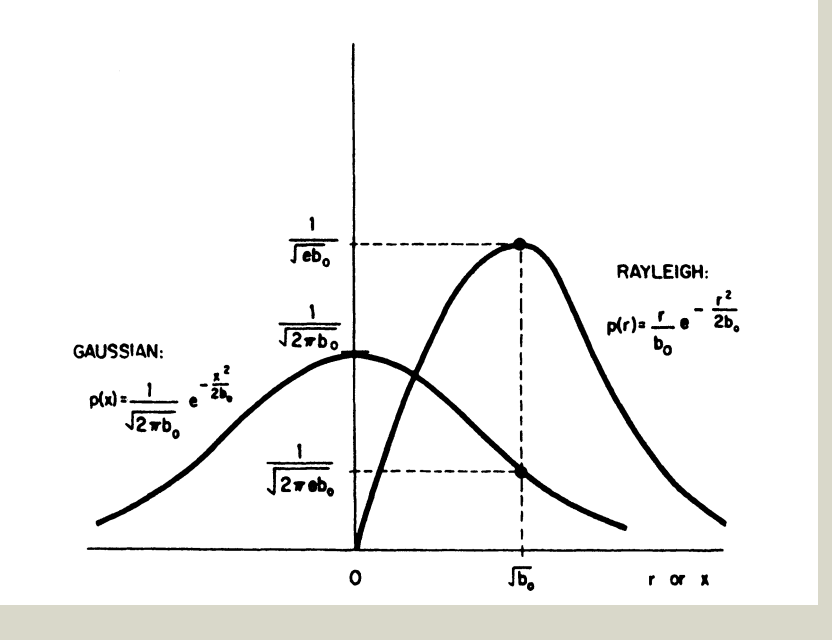
\includegraphics[width=\linewidth]{./Figures/%
	WirelessChannel/RayleighDistribution.png}
	\caption{Gaussian and Rayleigh Distributions%
	\cite{Jakes74}}
	\label{fig:RayleighDistribution}
\end{figure}

% TODO: Explain the rician v parameter
% it comes from the expression describing the K parameter
\begin{figure}[h!]
	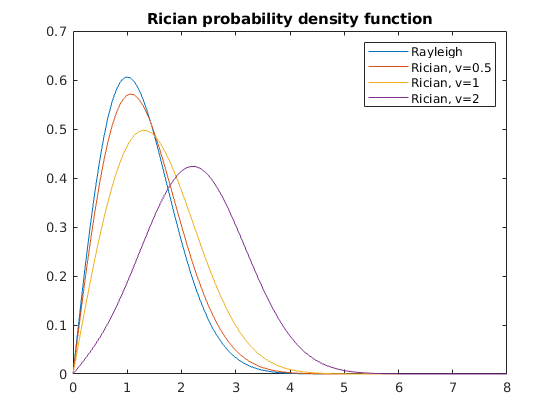
\includegraphics[width=\linewidth]{./Figures/%
	WirelessChannel/RicianDistribution.png}
	\caption{Rayleigh and Rician Distributions}
	\label{fig:RicianDistribution}
\end{figure}

% TODO: make a diagram of the Rician distribution
% TODO: Enter the expressions for a Rayleigh distribution
% TODO: Enter the expressions for a Rician distribution
% TODO: find and plot a measured Rayleigh distribution

Good modeling and simulation of this small scale fading %
is crucial to the accurate simulation of wireless channels. %
There are two main methods of simulating small scale fading, %
the sums of sinusoids method first developed by Jakes in %
\cite{Jakes74} and a filtered white gaussian noise method. %
The filtered white gaussian noise methodology is the chosen %
method of simulation for this report.

\section{Wireless Channel as a Filter}

% TODO: Develop Finite impulse response filter model 
% of the wireless channel

% TODO: develop the model for the time-varying characteristics
% of wireless channels

% TODO: Develop the mathematics of the finite gaussian channel model


